\documentclass[]{pfBook}

\renewcommand{\title}{SortSimulation}
\renewcommand{\subtitle}{Documentation}
\renewcommand{\author}{-- English --}
\renewcommand{\copyright}{Copyright \textcopyright{} 2008--2014 Peter Folta. All rights reserved.}

\newcommand{\version}{2.0.0 Alpha}
\newcommand{\URL}{\href{http://www.peterfolta.net/software/sortsimulation}{http://www.peterfolta.net/software/sortsimulation}}

\renewcommand{\belowtitle}{
	Version \version\newline{}
	Internet: \URL
}

\newcommand{\OO}{\mathcal{O}}

\begin{document}
	\pagenumbering{roman}
	\maketitlepage
	\cleardoublepage
	\maketableofcontents
	\cleardoublepage
	\pagenumbering{arabic}
	
	\section{Introduction}
	
	SortSimulation is a Java application that provides visual representations of different sorting algorithms. This gives users a better understanding of the various operating modes of said algorithms. The application is also useful for demonstrating the runtime differences \review{without simply comparing numbers}.
	
	\begin{figure}[h]
		\centering
		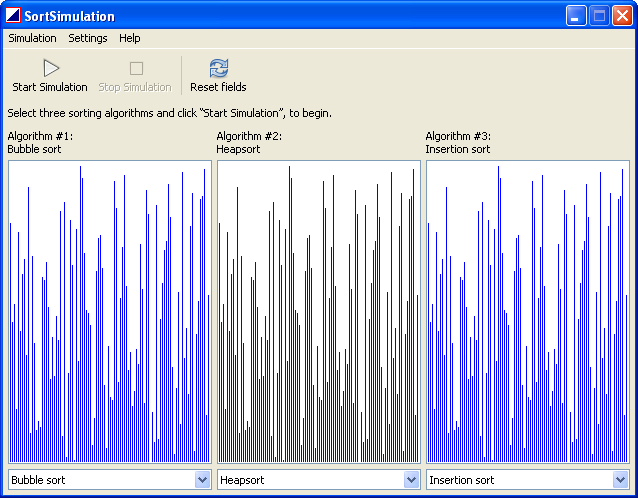
\includegraphics[scale=0.6]{images/image0.png}
		\caption{The main window of SortSimulation}
	\end{figure}
	
	This documentation contains a brief insight into the usage of SortSimulation and presents the supported sorting algorithms, including their java implementation.
	
	\section{Usage}
	
	Using SortSimulation is really simple: The sorting fields are randomly filled immediately after the launch of the program---every field contains the same initial situation. Three sorting algorithms are preselected also following the program launch.
	
	To compare the three particular sorting algorithms of your choice, select them from the combo boxes below the fields. Click on \emph{Start simulation} in the toolbar or the menu, or press the enter key on your keyboard alternatively, to begin. Cancelling an active simulation is just as easy: Press the escape key or click on \emph{Stop simulation}. To reset the fields after a finished or cancelled simulation, click on the button \emph{Reset fields} or press \texttt{Ctrl+N}.
	
	SortSimulation allows you to configure the simulation as you wish. The available settings are discussed in the following paragraph.
	
	\subsection{Settings}
	
	SortSimulation offers you miscellaneous options to configure the sorting simulations in the way you want it. The available settings are listed in the menu \emph{Settings}:
	
	\begin{figure}[h]
		\centering
		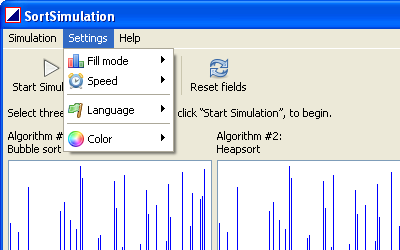
\includegraphics[scale=0.6]{images/image1.png}
		\caption{The settings menu}
	\end{figure}
	
	To configure the way the sorting fields are filled, the option \emph{Fill mode} offers you four possibilities: Randomly (preselected; \texttt{Ctrl+R}), Inverse (\texttt{Ctrl+I}), Almost sorted (\texttt{Ctrl+A}) and Presorted (\texttt{Ctrl+P}). If \emph{Randomly} is selected, the elements are ordered randomly in the fields when the user commits the action \emph{Reset fields}. This allows you to try the different sorting algorithms on totally unsorted data in a realistic way.
	
	In contrast, the mode \emph{Inverse} fills the fields already sorted---but backwards (descending instead of ascending). Using this setting gives you the possibility to take a closer look on the efficiency of the algorithms sorting backwards pre-ordered series.
	
	The mode \emph{Almost sorted} generates a randomly sorted sequence that only differs slightly from its real order. The rough structure of the sorted data is already recognizable. This options helps to visualize which sorting algorithms are particularly useful for sorting data sets that only marginally differ from their sorted order.
	
	The last option \emph{Presorted} fills all fields with already sorted data. This might be useful for understanding how different sorting algorithms work on an already sorted set of data.
	
	The submenu \emph{Speed} allows you to configure the speed of the simulation. You can choose the speed between five levels. While algorihms like Bubble sort are quite slow, it is worth to select one of the higher speed levels; while running a sorting algorithm like Quicksort, it's better to choose a slower speed to be able to take a closer look at the functionality. It's also possible to set the different speed levels by keyboard using the sortcuts \texttt{Ctrl+Shift+(1-5)}.
	
	SortSimulation doesn't create or modify any of the files stored on your computer, that's why SortSimulation's user interface language is always set to English after the program launch, even if you changed it before. To switch between the offered languages, go to the submenu \emph{Language}.
	
	The last two sub menus \emph{Background} and \emph{Color} allow you to change the color of the bars as well as to adjust the background color of the panes.
	
	\subsection{Parameter}
	\label{StartUpArguments}
	
	By default, SortSimulation displays three fields next to each other. This allows for the visualization of three sorting algorithms parallel to each other. By using a parameter at the program launch, you can adjust the amount of displayed fields. To do that, simply provide the desired amount. Valid values are between 2 and 9.
	
	To launch SortSimulation with 5 fields for instance, please run the following command from a terminal window:
	
	\begin{lstlisting}[style=shell]
SortSimulation 5
	\end{lstlisting}
	
	SortSimulation will continue to start as usual, but shows the provided 5 fields this time instead of the default 3:
	
	\begin{figure}[h]
		\centering
		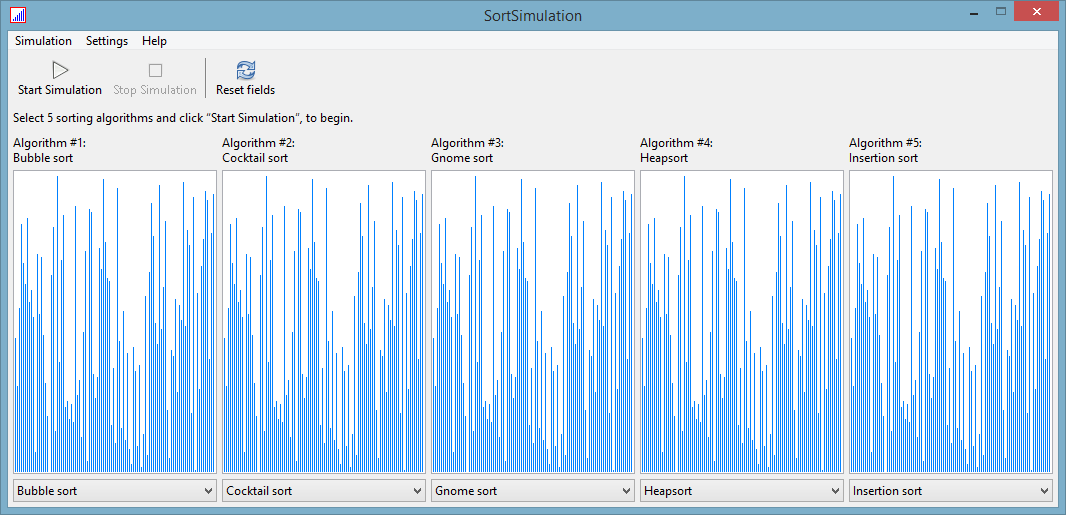
\includegraphics[scale=0.6]{images/image2.png}
		\caption{SortSimulation with 5 fields}
		\label{fig:5fields}
	\end{figure}
	
	Please note when using this method that SortSimulation's main window may become very wide and might be bigger than your what your screen is able to display.
	
	If you provide an invalid value, you will receive the following error message:
	
	\begin{figure}[h]
		\centering
		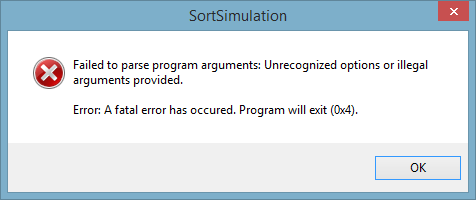
\includegraphics[scale=0.6]{images/image3.png}
		\caption{Error message when using illegal parameters}
		\label{fig:parameterserror}
	\end{figure}
	
	\section{Sorting algorithms}
	
	\subsection{Bubble sort}
	
	Bubble sort is a really simple sorting algorithm, that sorts elements using a \emph{step-by-step comparison}. Because bubble sort is not very efficient, it is often used to demonstrate a weak sorting algorithm.
	
	\subsubsection{Idea of Bubble sort}
	
	Bubble sort works by comparing two list items and swapping them if they are in the wrong order. This procedure is repeated until all elements are in the correct position.
	
	\subsubsection{Performance}
	
	Bubble sort has typically complexity $\OO(n^2)$, where $n$ is the number of items being sorted. Performance of bubble sort over an already-sorted list (best-case) is $\OO(n)$.
	
	\subsubsection{Java implementation}
	
	\lstinputlisting[caption={Implementation of Bubble sort}, label=lst:bubblesort, style=java]{../listings/Bubblesort.java}
	
	\subsection{Cocktail sort}
	
	Cocktail sort, also known as \emph{Shaker sort}, is a simple sorting algorithm, which is a variant of the popular bubble sort.
	
	\subsubsection{Idea of Cocktail sort}
	
	The to be sorted sequence of elements is being iterated upwards and downwards alternatingly. In each step, two neighboring elements are being compared and swapped if they are in the wrong order. Because of this, a cluster of large elements forms on the upper end of the array and a cluster of small elements form on the lower end.
	
	\subsubsection{Performance}
	
	Cocktail sort has typically complexity $\OO(n^2)$, where $n$ is the number of items being sorted. It strives towards $\OO(n)$ for almost sorted sequences.
	
	\subsubsection{Java implementation}
	
	\lstinputlisting[caption={Implementation of Cocktail sort}, label=lst:cocktailsort, style=java]{../listings/Cocktailsort.java}
	
	\subsection{Gnome sort}
	
	Gnome sort is a very simple sorting algorithm, that sorts elements by \emph{step-by-step comparison}. It was originally proposed by \emph{Hamid Sarbazi-Azad} in 2000 under the name \emph{Stupid Sort}. Later the name was changed into Gnome sort. Gnome sort has the advantage of requiring just one loop (and thus no nested loops).
	
	\subsubsection{Idea of Gnome sort}
	
	Gnome sort works in a way one might imagine a garden gnome: Suppose a garden gnome wants to sort flower pots. He initially stands at the left end of the sequence of pots. The gnome compares two neighboring flower pots: If they are in correct order, he moves one pot to the right. If they are not, he swaps them and makes one step to the left, unless he is standing at the left end of the pot sequence. In that case, the garden gnome makes one step to the right. This procedure is repeated until he gets to the right end of the sequence (and therefore reaches the last flower pot).
	
	\subsubsection{Performance}
	
	Gnome sort has typically complexity $\OO(n^2)$, where $n$ is the number of items being sorted. It strives towards $\OO(n)$ for almost sorted sequences.
	
	\subsubsection{Java implementation}
	
	\lstinputlisting[caption={Implementation of Gnome sort}, label=lst:gnomesort, style=java]{../listings/Gnomesort.java}
	
	\subsection{Heapsort}
	
	Heapsort is a fast sorting algorithm which was developed by \emph{Robert W. Floyd} and \emph{J.\,W.\,J. Williams} in 1964. Heapsort is an improvement of \emph{Selection sort}.
	
	\subsubsection{Idea of Heapsort}
	
	Heapsort uses the \emph{heap} as a specialized data structure for sorting. This data structure is based on an (almost) complete \emph{binary tree}. A binary tree is (almost) complete, if all levels except possibly the last are completed.
	
	If the sequence exists as a heap, the largest element can be taken out of the \emph{root} of the tree. To get to the next item, the heap has to be \emph{rearranged} before.
	
	\subsubsection{Performance}
	
	Heapsort always has complexity $\OO(n \log n)$ and is therefore one of the best comparison sorts.
	
	\subsubsection{Java implementation}
	
	\lstinputlisting[caption={Implementation of Heapsort}, label=lst:heapsort, style=java]{../listings/Heapsort.java}
	
	\subsection{Insertion sort}
	
	Insertion sort is a quite simple sorting algorithm. It is not as efficient as other more complex algorithms, but \emph{easy to implement} and has a very short run time in case of a small amount of data or already presorted data.
	
	\subsubsection{Idea of Insertion sort}
	
	Insertion sort removes an element of the unsorted set and inserts it in the correct place of the output sequence. If the sequence is empty, the element will be inserted at the first position.
	
	Insertion sort is inefficient, because this sorting algorithm often needs to move elements over long distances.
	
	\subsubsection{Performance}
	
	Insertion sort has typically complexity $\OO(n^2)$, where $n$ is the number of items being sorted. It strives towards $\OO(n)$ for almost sorted sequences.
	
	\subsubsection{Java implementation}
	
	\lstinputlisting[caption={Implementation of Insertion sort}, label=lst:insertionsort, style=java]{../listings/Insertionsort.java}
	
	\subsection{Merge sort}
	
	Merge sort is a recursive and stable sorting algorithm, which is based on the \emph{divide and conquer principle}, like \emph{Quicksort}. Merge sort was presented by John von Neumann in 1945.
	
	\subsubsection{Idea of Merge sort}
	
	Merge sort splits the sequence into several smaller sequences, which will be sorted each for itself. After that the sorted, small sequences are united in one completly sorted sequence.
	
	\subsubsection{Performance}
	
	Merge sort always has complexity $\OO(n \log n)$ and is therefore one of the best comparison sorts.
	
	\subsubsection{Java implementation}
	
	\lstinputlisting[caption={Implementation of Merge sort}, label=lst:mergesort, style=java]{../listings/Mergesort.java}
	
	\subsection{Quicksort}
	
	Quicksort is one of the \emph{fastest sorting algorithms}, based on the \emph{divide and conquer principle}. The recursive Quicksort algorithm in its original version was developed by \emph{C. Antony R. Hoare} in 1960.
	
	\subsubsection{Idea of Quicksort}
	
	The sequence will initially be split into two part. The first section contains all elements less than or equal to all elements in the second section (\emph{divide}). Then the two pieces are independently recursively sorted using the same procedure (\emph{conquer}). The last step combines the smaller sequences to a sorted one (\emph{combine}).
	
	The division is realized using a \emph{pivot element}, which is selected from the array in the first step. All elements of the sequence, which are \emph{smaller} than the pivot element, will be put in the first section. All the elements, that are \emph{larger} than the pivot element, will be put in the second section. For elements which have the same value as the pivot element, it does not matter in what part they are put.
	
	\subsubsection{Performance}
	
	Quicksort has typically complexity $\OO(n \log n)$, where $n$ is the number of items being sorted. It is therefore one of the best comparison sorts. The worst case performance of Quicksort has complexity $\OO(n^2)$.
	
	\subsubsection{Java implementation}
	
	\lstinputlisting[caption={Implementation of Quicksort}, label=lst:quicksort, style=java]{../listings/Quicksort.java}
	
	\subsection{Selection sort}
	
	Selection sort is a naive sorting algorithm that works in place. It is compareable to insertion sort.
	
	\subsubsection{Idea of Selection sort}
	
	Selection sort divides the sequence in a \emph{sorted} and a \emph{unsorted} field. The sorted part is empty at the beginning. Selection sort examines the smallest element in the unsorted part and swaps it with the first element. The sequence is sorted until this position after the step is made. The procedure is repeated until the entire sequence is sorted.
	
	\subsubsection{Performance}
	
	Selection sort always has complexity $\OO(n^2)$.
	
	\subsubsection{Java implementation}
	
	\lstinputlisting[caption={Implementation of Selection sort}, label=lst:selectionsort, style=java]{../listings/Selectionsort.java}
	
	\subsection{Shell sort}
	
	The sorting algorithm Shell sort is based on \emph{Insertion sort}. It was invented in 1959 by \emph{Donald L. Shell}.
	
	\subsubsection{Idea of Shellsort}
	
	Shellsort compensates the disadvantage of Insertion sort to move elements over large distances. Shellsort creates a \emph{k-column matrix}, whose columns are sorted separately. After these steps, the result is already sorted coarse. The step is repeated every time while the number of columns is reduced, until the matrix consists of only a single column.
	
	\subsubsection{Performance}
	
	Shell sort has best case complexity $\OO(n \log n)$ and worst case complexity $\OO(n^2)$. The average case is in between and has complexity $\OO(n \log^2 n)$.
	
	\subsubsection{Java implementation}
	
	\lstinputlisting[caption={Implementation of Shell sort}, label=lst:shellsort, style=java]{../listings/Shellsort.java}
	
	\section{Contributors}
	
	This is to thank the following persons, who have vigorously supported the development of SortSimulation. New contributors (translators, designers, writers of documentation, etc.) are needed constantly~-- if you are interested in contributing, please get in touch with Peter Folta.\\
	[\baselineskip]
	Allison, Chloë Louise\\
	Folta, Lucia Sonja\\
	Folta, Peter\\
	Müllner, Jan Sebastian
	
	\begin{thebibliography}{99}
		\bibitem{Lang}
			\textsc{Lang}, Prof. Dr. Hans Werner: \emph{Algorithmen in Java}. 2nd Edition 2006. Munich: Oldenbourg Wissenschaftsverlag GmbH 2006. ISBN 978-3-486-57938-3, pp.~5--52
		\bibitem{Sarbazi}
			\textsc{Sarbazi-Azad}, Dr. Hamid: \emph{Stupid Sort: A new sorting algorithm}. In: \emph{Department of Computer Science Newsletter, University of Glasgow}. No. 4, October 2, 2000. \href{http://sina.sharif.edu/~azad/stupid-sort.PDF}{http://sina.sharif.edu/\~{}azad/stupid-sort.PDF}
	\end{thebibliography}
	
	\makelistoffigures
	\makelistoflistings
\end{document}